
%(BEGIN_QUESTION)
% Copyright 2010, Tony R. Kuphaldt, released under the Creative Commons Attribution License (v 1.0)
% This means you may do almost anything with this work of mine, so long as you give me proper credit

Determine the value of the specified {\it integral} for this function:

$$\includegraphics[width=15.5cm]{i04382x01.eps}$$

$$\int_{-9}^{-3} y \> dx$$

\vskip 20pt \vbox{\hrule \hbox{\strut \vrule{} {\bf Suggestions for Socratic discussion} \vrule} \hrule}

\begin{itemize}
\item{} What is most important when solving problems such as this is to be able to explain {\it why} (not just {\it how}) to arrive at the correct value.  Try explaining the process of integration in your own words, as it applies to this particular problem.
\item{} Identify the mathematical sign of the function ($y$) and of the differential ($dx$) over various portions of the integration interval (as $x$ varies between $-9$ and $-3$).  Are there places where $y$ changes sign?  Are there places where $dx$ changes sign?
\end{itemize}

\underbar{file i04382}
%(END_QUESTION)





%(BEGIN_ANSWER)

+0.5

%(END_ANSWER)





%(BEGIN_NOTES)


%INDEX% Mathematics, calculus: integral (approximating integral values between points on graph)

%(END_NOTES)


